\documentclass[12pt]{article}
\usepackage[margin=3cm]{geometry}
\geometry{a4paper}
\usepackage[parfill]{parskip}
\usepackage{mathtools}

\usepackage{caption}

\begin{document}

\begin{center}
    \huge{Yong Shen Tan}\\
    \vspace{0.3cm}
    \large{CID: 01055349}\\
    \vspace{0.3cm}
    \large{Reinforcement Learning (Second Half) Coursework}\\
    \vspace{0.3cm}
\end{center}

\vspace{1.5cm}

\textbf{Question 1 (i)}
As seen from the variance of the loss curves in Figures 1 (a) and (b), mini-batch learning results in more stable training of the Q-network. This is because in online learning we are taking the Q-network's loss of a single transition, whereas in mini-batch learning we are averaging the loss over multiple transitions, thus leading to higher precision in Q-value predictions. Furthermore, in mini-batch learning the randomly sampled transitions used to train the Q-network is more evenly distributed across the environment, resulting in more stable learning.
\vspace{0.5cm}

\textbf{Question 1 (ii)}
Training the Q-network using mini-batch learning is more efficient at improving its predictive accuracy per episode of interaction. This is because in mini-batch learning we are feeding our neural network with more transition data, allowing it to better learn and optimise its weights leading to more accurate predictions. Furthermore, as transitions are stored in a replay buffer rather than discarded upon training, the agent doesn't have to revisit state-action pairs to train on those transitions.

\vspace{2cm}
\textbf{Question 2 (i)}
Yes, it is likely that the Q-value predictions for the bottom-right corner are more accurate than the ones for the top-right corner. Given that the agent only takes 20 random steps per episode and is in closer proximity to the bottom-right corner, it is highly likely to have experienced more transitions in the bottom-right corner than in the top-right. This means that sampling from our replay buffer will result in more transitions from the former for the Q-network to train on, and is thus able to more accurately predict their Q-values.

\vspace{0.5cm}
\textbf{Question 2 (ii)}
Based on the greedy policy seen in Figure 2 (b), the agent would not reach the goal if it were to execute this policy. With a discount factor of 0, the Q-network is myopic and only takes into account immediate rewards when predicting Q-values. This means that the highest predicted reward the agent can get is by going straight up towards the goal and be blocked by the obstacle, as moving anywhere but up will lead to less immediate reward.


\vspace{2cm}
\textbf{Question 3 (i)}
Applying the Bellman equation with a discount factor of 0.9, the Q-network is now far-sighted and takes into account the discounted sum of future rewards. Given sufficient exploration of the states in the upper half of the environment near the goal, the agent is now able to learn that going around the obstacle and getting to the goal, despite lesser immediate rewards than staying at the wall, will allow it to maximise the overall rewards it obtains in the long-term.

\vspace{0.5cm}
\textbf{Question 3 (ii)}
After introducing the target network, the loss is now being calculated using the target network's prediction for the Bellman equation rather than the Q-network's. As the target network remains stationary until we update its weights using the Q-network's weights every 10 episodes, we see that the Q-network's loss decreases and stablises every 10 episodes, but drastically increases afterwards as the target network is now predicting Q-values based off its newly updated weights. The Q-network thus has to learn and readjust its weights to decrease this prediction error. This accounts for the spikes in the loss curve seen in Figure 3 (b).

\vspace{2cm}
\textbf{Question 4 (i)}
It is not possible for the agent to ever reach the goal if \(\epsilon\) was always zero. An \(\epsilon\) of zero means the agent always adopts a greedy policy and chooses the action which results in the highest Q-value, without doing any exploration of states that can possibly lead to better rewards. In this case, the greedy policy is a sub-optimal one based on how the Q-network's weights were initialised, and exploiting this policy leads to the agent getting stuck between states as its not able to learn better Q-values without exploring.

\vspace{0.5cm}
\textbf{Question 4 (ii)}
Before the Q-network has converged it is possible that the agent has not  sufficiently explored the states to the left of the goal to accurately predict their Q-values; the Q-network might incorrectly predict higher Q-values for those states compared to the goal state as it has not been trained on those transitions sufficiently. This results in a greedy policy where the agent will continue moving left after reaching the goal as it assumes it can obtain better rewards by moving towards those states with higher Q-values.


\clearpage
\begin{figure}
    \centering
    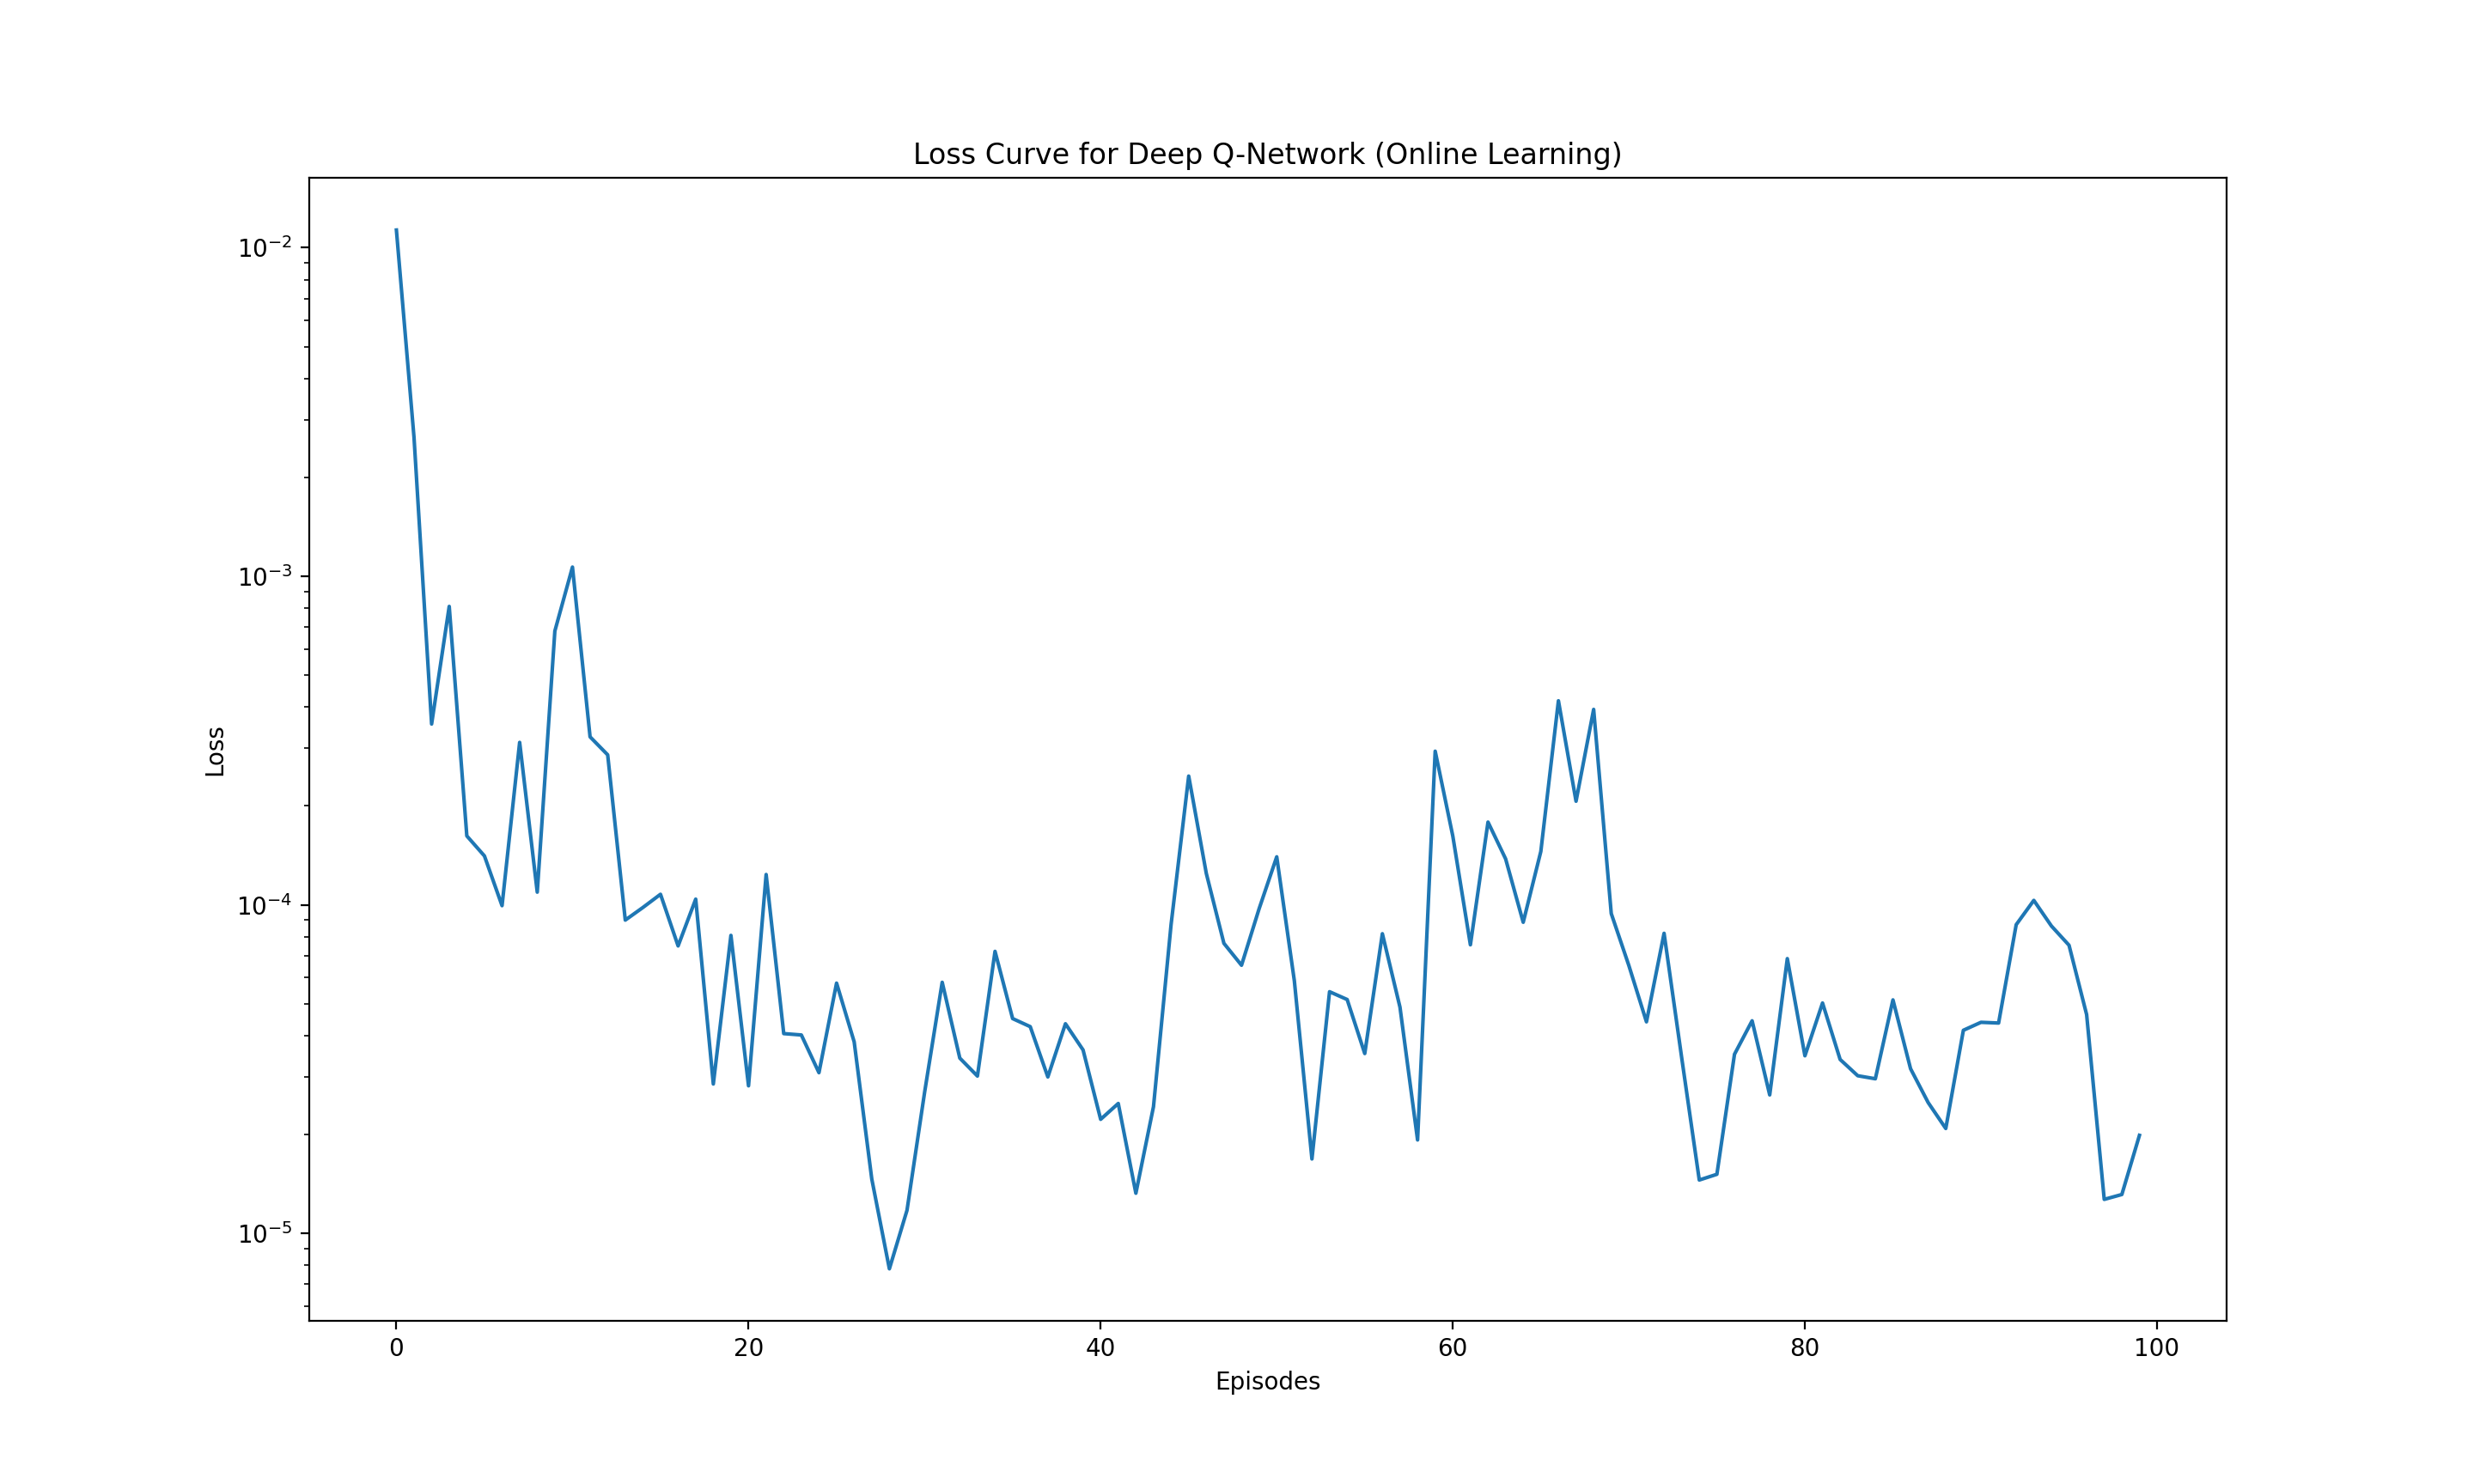
\includegraphics[width=15cm]{figures/1a.png}
    \caption*{Figure 1 (a): Deep Q-network Loss Curve with Online Learning}
\end{figure}
\begin{figure}
    \centering
    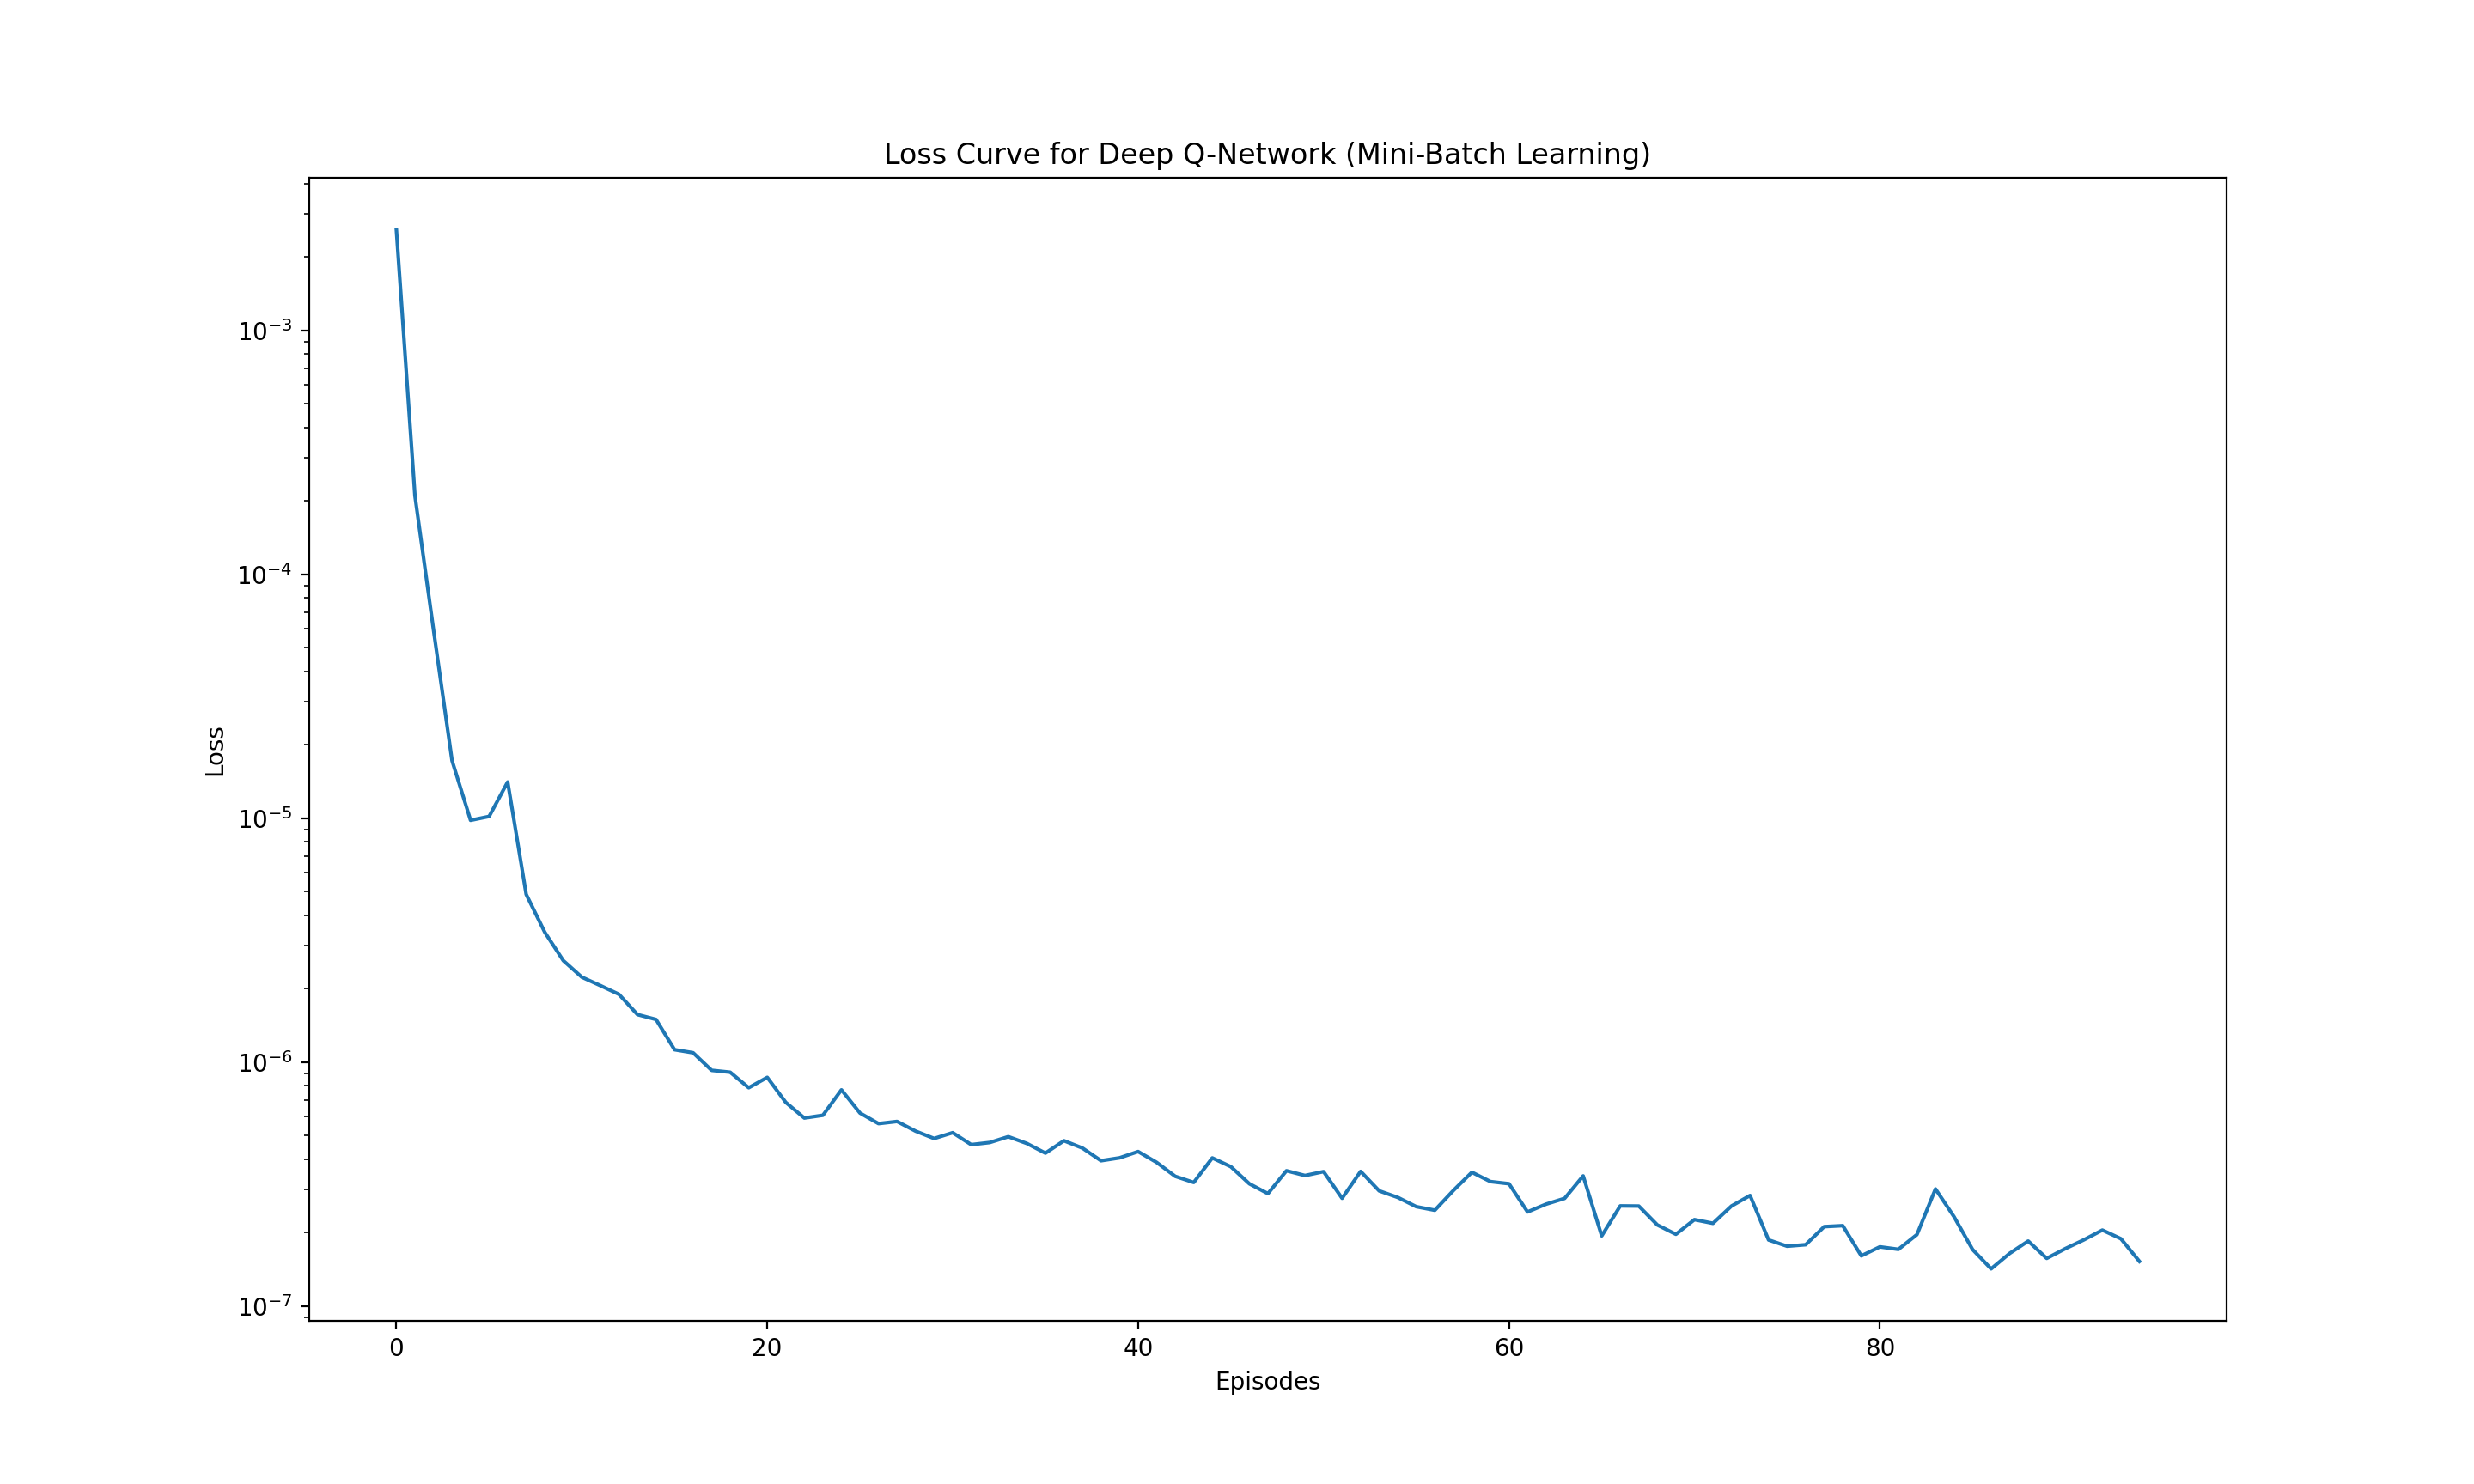
\includegraphics[width=15cm]{figures/1b.png}
    \caption*{Figure 1 (b): Deep Q-network Loss Curve with Mini-Batch Learning}
\end{figure}

\clearpage
\begin{figure}
    \centering
    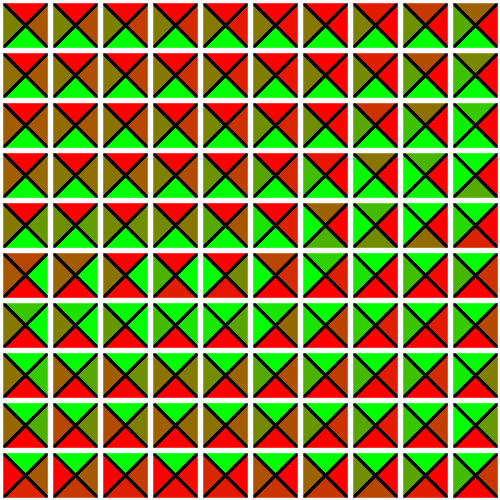
\includegraphics[width=10cm]{figures/2a.png}
    \caption*{Figure 2 (a): Visualisation of Q-values}
\end{figure}
\begin{figure}
    \centering
    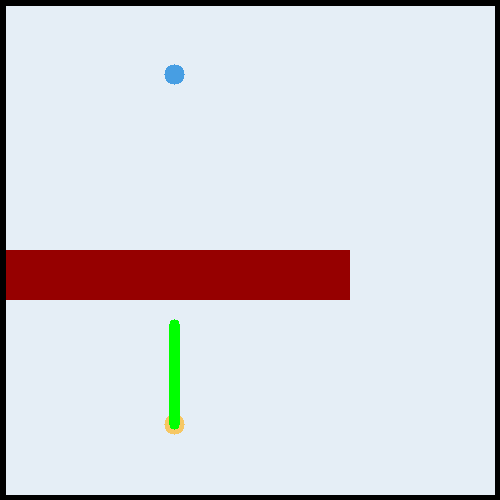
\includegraphics[width=10cm]{figures/2b.png}
    \caption*{Figure 2 (b): Visualisation of Greedy Policy}
\end{figure}

\clearpage
\begin{figure}
    \centering
    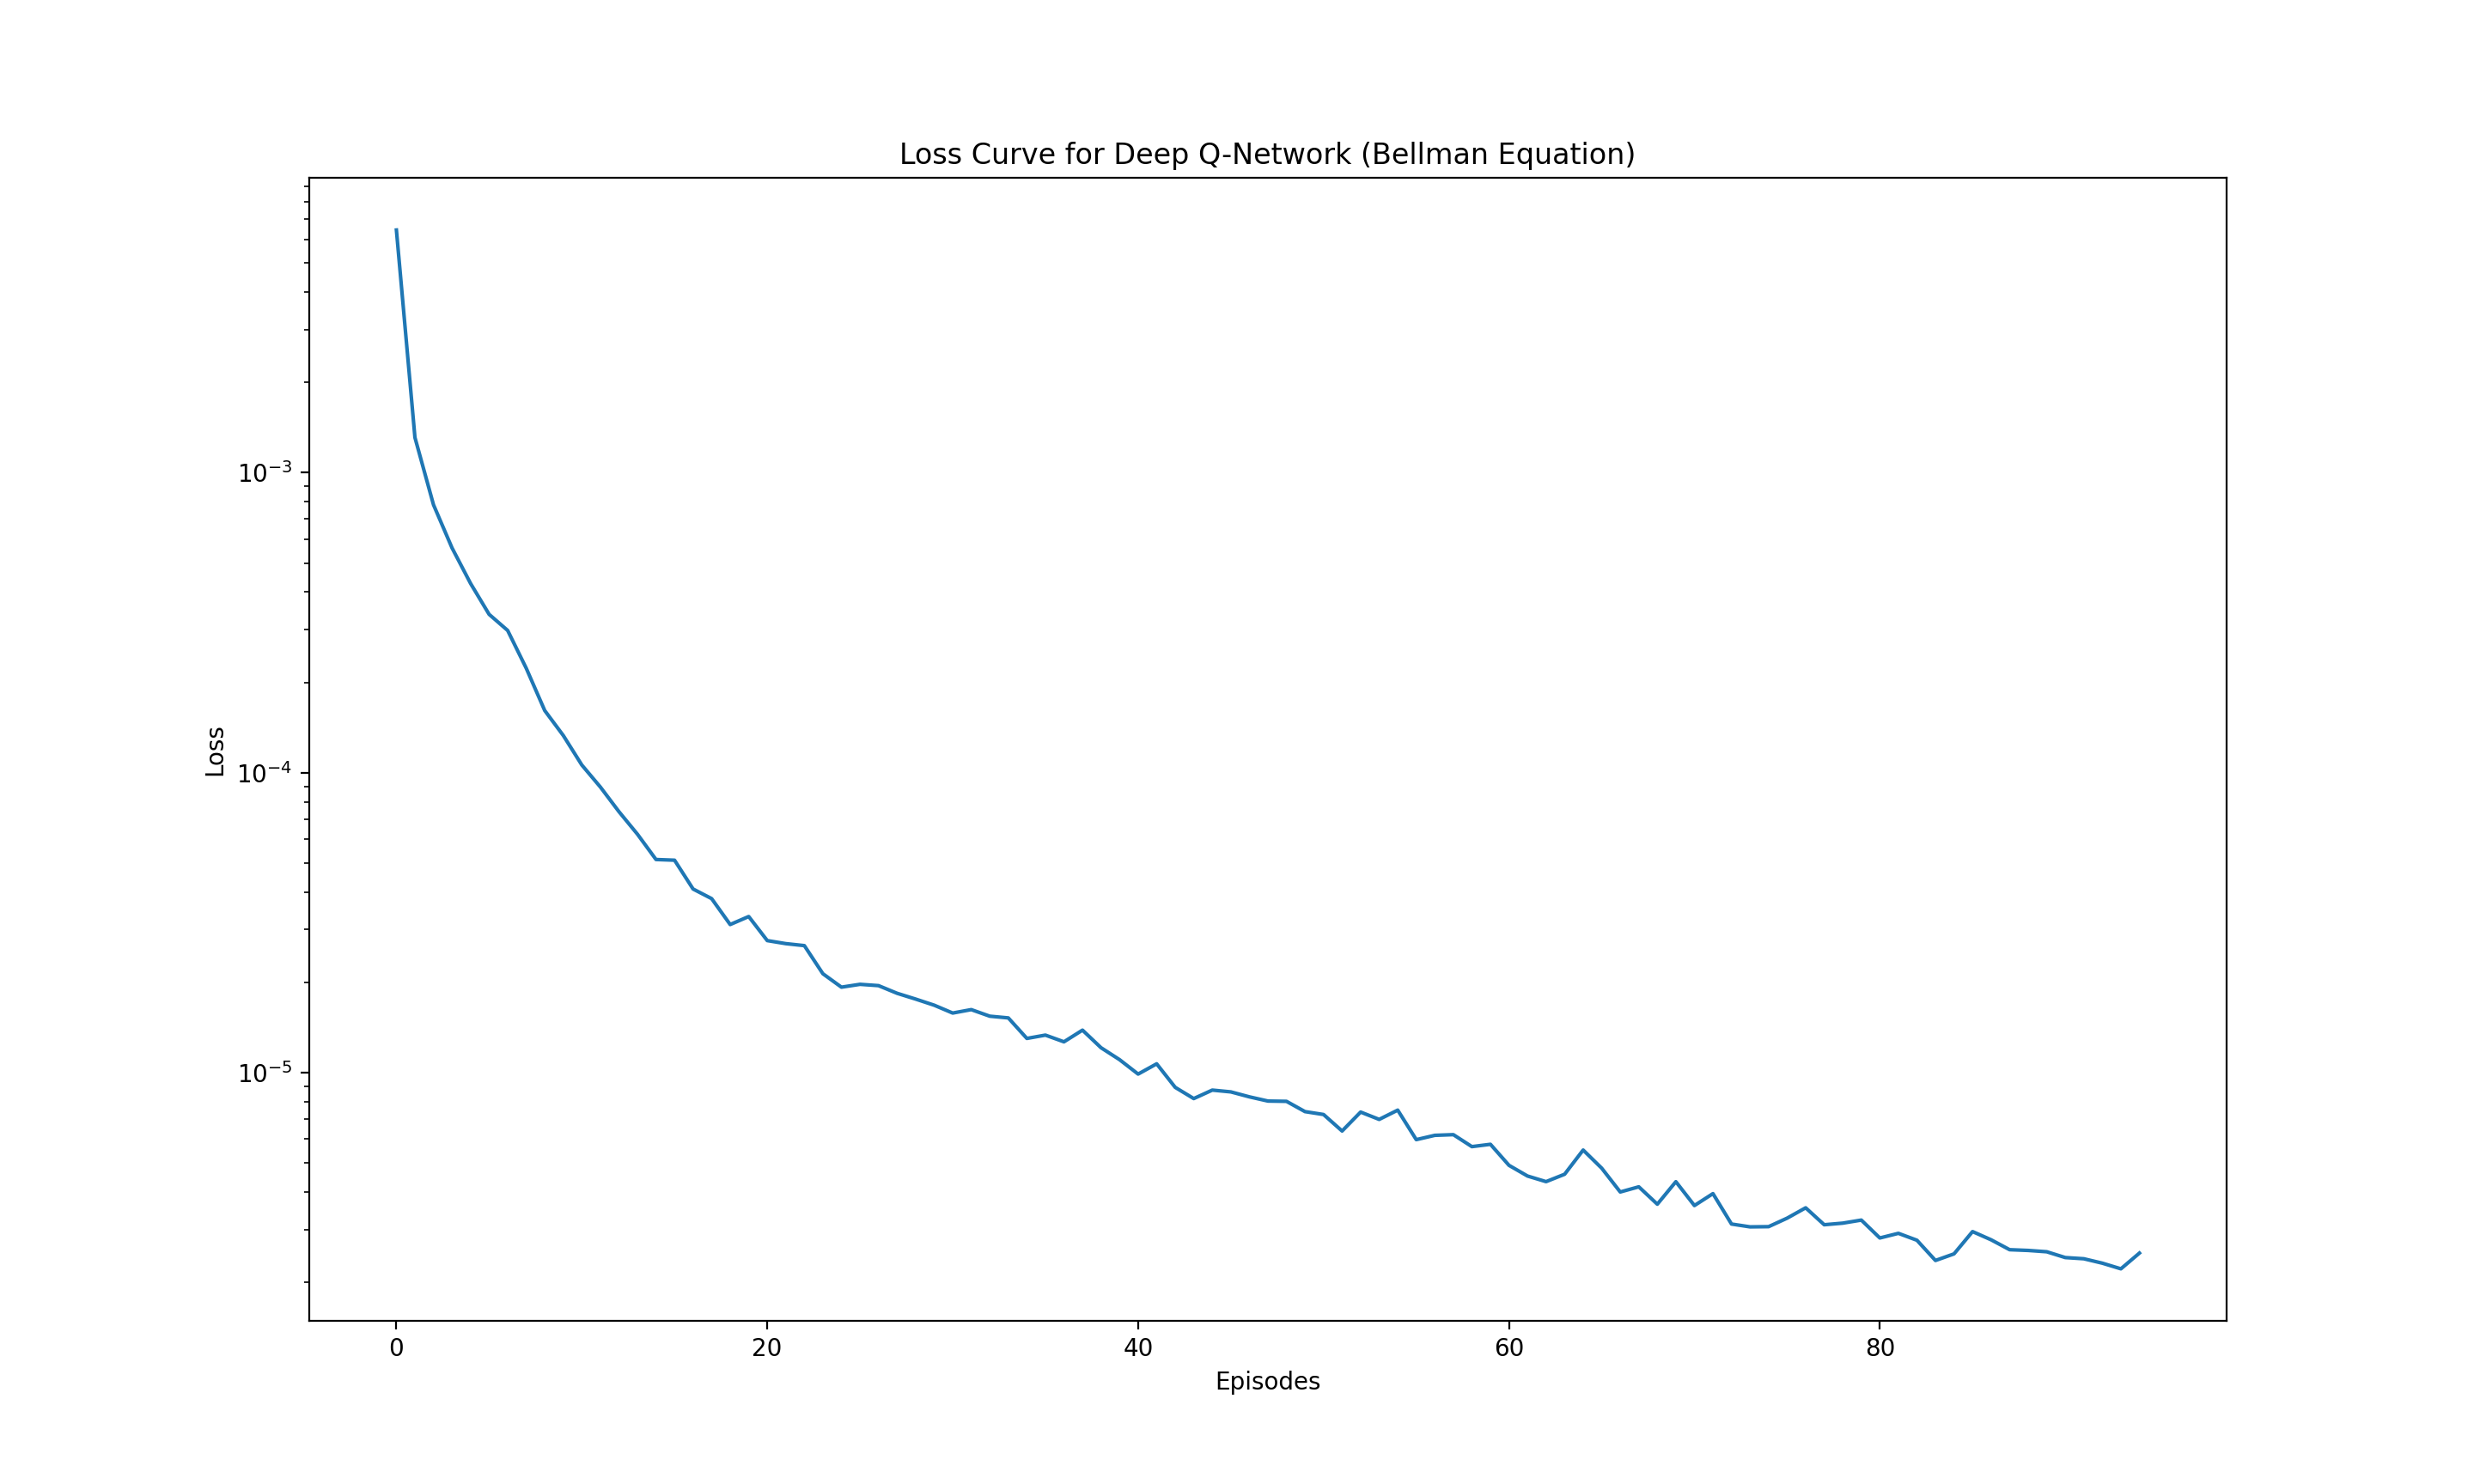
\includegraphics[width=15cm]{figures/3a.png}
    \caption*{Figure 3 (a): Deep Q-network Loss Curve with Bellman Equation}
\end{figure}
\begin{figure}
    \centering
    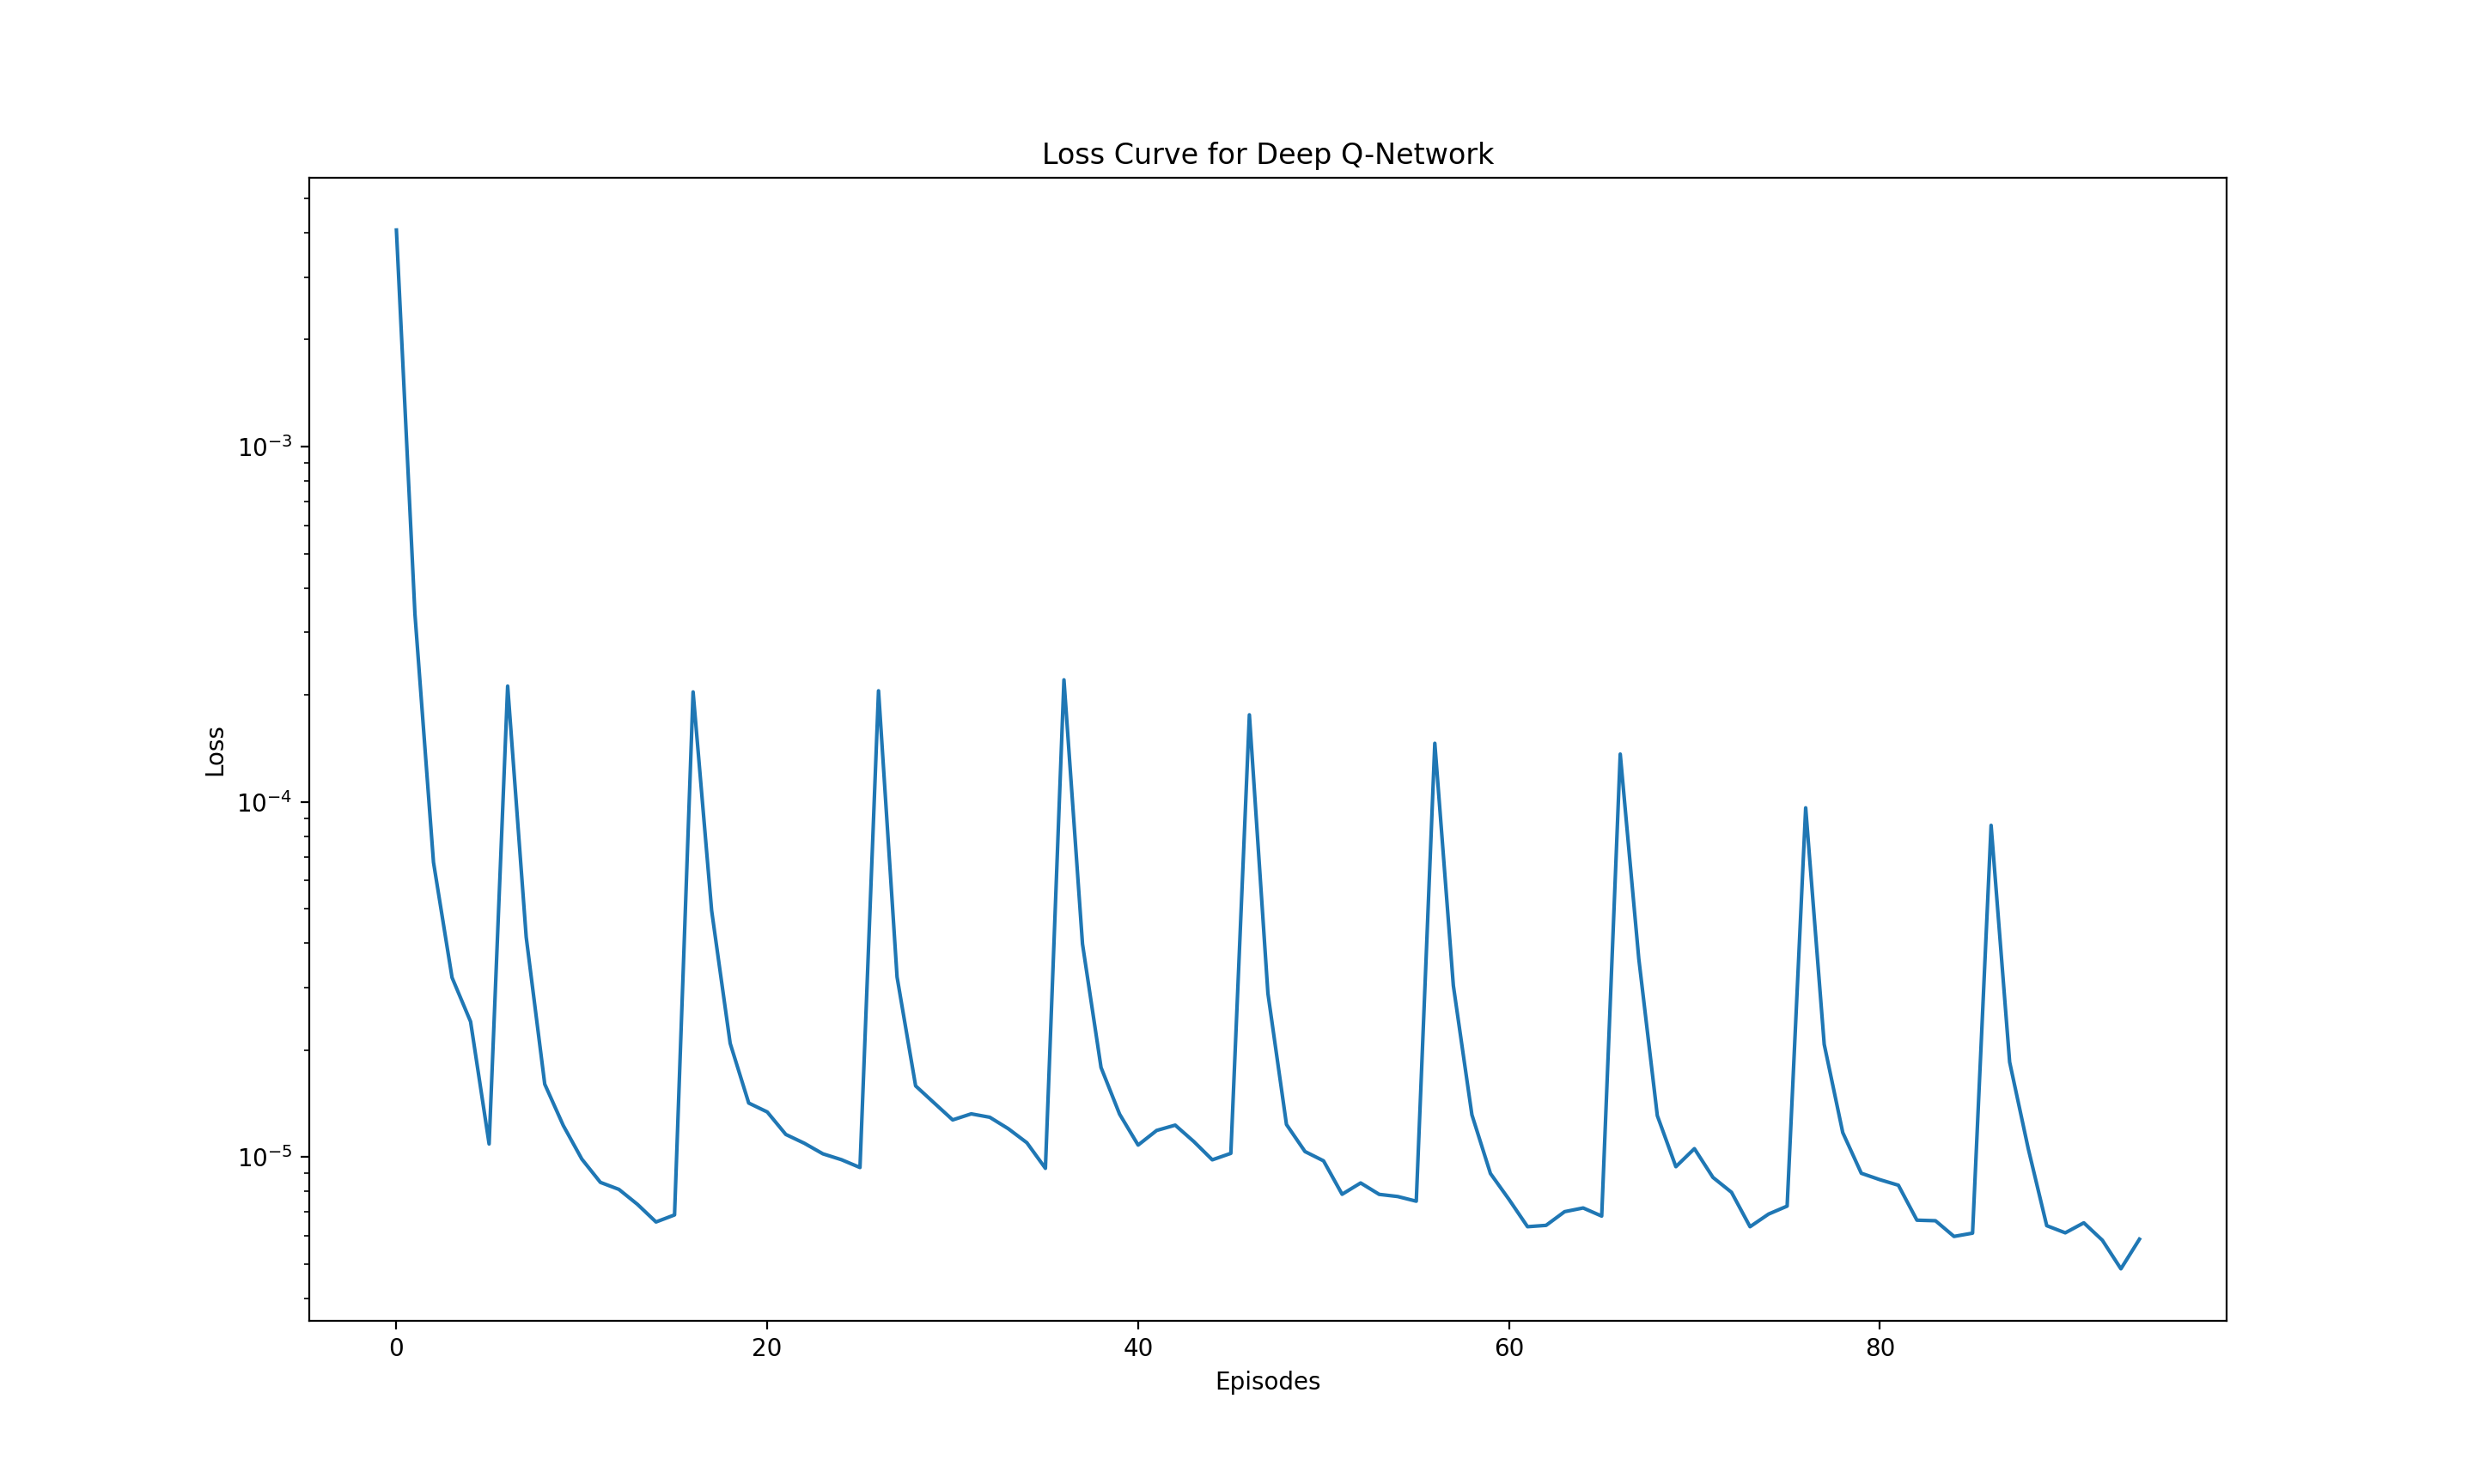
\includegraphics[width=15cm]{figures/3b.png}
    \caption*{Figure 3 (b): Deep Q-network Loss Curve with Target Network}
\end{figure}

\clearpage
\begin{figure}
    \centering
    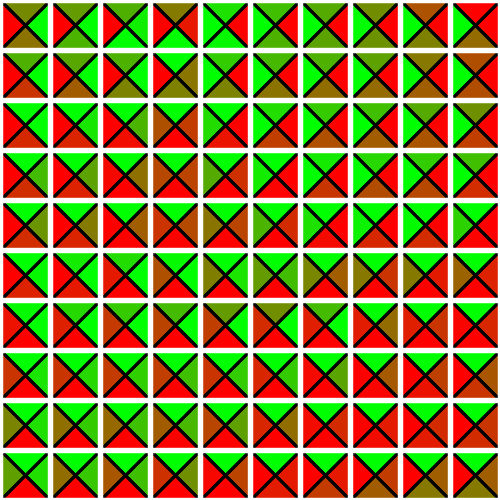
\includegraphics[width=10cm]{figures/4a.png}
    \caption*{Figure 4 (a): Visualisation of Q-values}
\end{figure}
\begin{figure}
    \centering
    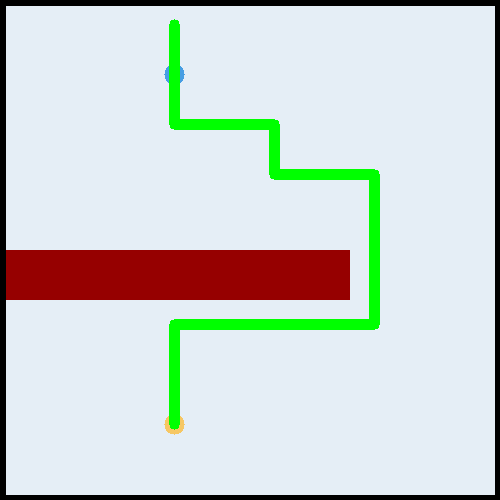
\includegraphics[width=10cm]{figures/4b.png}
    \caption*{Figure 4 (b): Visualisation of Greedy Policy}
\end{figure}

\clearpage
\newpage 

\begin{center}
    \large{Description of Implementation for Part 2}
\end{center}
\vspace{1cm}
To help the agent learn to navigate the environment and get to the goal, a \textbf{DQN} class is created to represent a deep Q-network. This class initialises (\textit{L12-22}) a Q-network whose weights get optimised during training, as well as a target network for more stable learning. Both networks are identical (\textit{L79-99}): an input dimension of 2 for state, an output dimension of 4 to represent discrete actions, 2 hidden linear layers with a ReLU activation function, and a linear output layer. The \textbf{DQN} class exposes a \textbf{train} method for training the deep Q-network, given a minibatch of transitions and a discount factor \(\gamma\) (further explained below). To apply mini-batch learning on the agent for more efficient and stable learning, a \textbf{ReplayBuffer} class is defined that inherits from the \textbf{collections.deque} class (\textit{L102-104}). The \textbf{sample} method (\textit{L106-108}) returns a randomly sampled mini-batch of transitions of the requested size from the buffer (with uniform distribution and without replacement).

The \textbf{Agent} class is initialised (\textit{L111-146}) with both the above classes, using a learning rate of 0.001 and maximum length of 6000 respectively. Additionally, the following attributes are defined: an episode length of 300, a mini-batch size of 600, and a \(\gamma\) of 0.9. A decaying \(\epsilon\) is also used, with starting and minimum values of 1.0 and 0.1 respectively. The \textbf{get\_next\_action} method returns a continuous action to be taken for a given state. To decide this action (\textit{L154-161}), an \(\epsilon\)-greedy policy is used, where the discrete action with the highest predicted Q-value by the DQN is chosen with (\(1-\epsilon\)) probability. A discrete action between 0 and 3 is chosen randomly otherwise. This action is then converted to a continuous one (\textit{L214-226}) with a magnitude of 0.02, where 0 is right, 1 is up, 2 is left, and 3 is down.

In the \textbf{Agent}'s \textbf{set\_next\_state\_and\_distance} method, a reward is assigned to the agent (\textit{L177-188}) - if it is nearing the end of an episode, a negative reward is assigned with a small probability, proportional to its distance from the goal. Otherwise, it's assigned a reward of (\(1-distance\)). This helps the agent get out from being stuck in local maxima due to sub-optimal policies. This transition is then added to the replay buffer, which when full is sampled for a mini-batch and used to train the agent's DQN (\textit{L194-197}). Finally, every 300 steps the target network is updated using the Q-network's weights, and epsilon is decayed by a factor of 0.988 (\textit{L200-202}).

The DQN is trained using double deep Q-learning. Firstly, the Q-network's predicted Q-value for each transition's corresponding action is computed (\textit{L36-42}). The Q-network's predicted Q-value for each next state is also computed using each transition's corresponding action with the highest Q-value as predicted by the target network (\textit{L44-57}). The Bellman equation is then applied (\textit{L59-72}) using the latter set of Q-values to obtain the label data for computing the Q-network's mean-squared error against the former set of Q-values. The Q-network's weights are then optimised using this error value to improve its predictions.

To obtain the agent's final greedy policy, the \textbf{get\_greedy\_action} method (\textit{L204-211}) chooses the discrete action with the highest predicted Q-value by the DQN for the given state, and converts that to a continuous action as described above.

\end{document}